\clearpage
\section{Standard Model Backgrounds}\label{ZP_SM_background}
There are three main kinds of backgrounds for this analysis. The most important and irreducible one is the SM Drell-Yan process.

The second most important background type includes \ttbar\ and \ttbar\-like processes, which contain WW, WZ, ZZ, tW, and \ztt. The \ttbar is the dominant background comparing to the others. However, WW events become increasingly important at high mass. Indeed at high mass, the top and antitop are boosted. The top decay products are then collimated, the b jet is close to the electron from the W decay. In this case, the electron usually fails the isolation requirements, reducing the contribution of \ttbar background at high mass.

The third type of background is the jet background, where jets are misidentified as electrons. The jet background mainly comes from W+jets and multijets processes.

\subsection{SM Drell-Yan background}\label{sbusec:DY_xs}

The SM Drell-Yan background is estimated by MC simulation and the MC samples are normalized to the data in the Z boson peak region of 60-120 GeV. They are also corrected with the trigger turn on curve.

Figure~\ref{fig:Zpeak} shows the data and MC at the Z peak for the barrel-barrel and barrel-endcap regions. In this case, in order to see the normalisation agreement between data and MC, MC events are normalized to the luminosity. Besides, the trigger turn on curve is applied and the scale factors between data and MC for gsf electron reconstruction efficiency and HEEP ID efficiency are applied. Further to this, the official EGamma corrections for electron energy scale and smearing are applied to data and MC in order to get better data and MC agreement.


\begin{figure}[bh]
\begin{center}
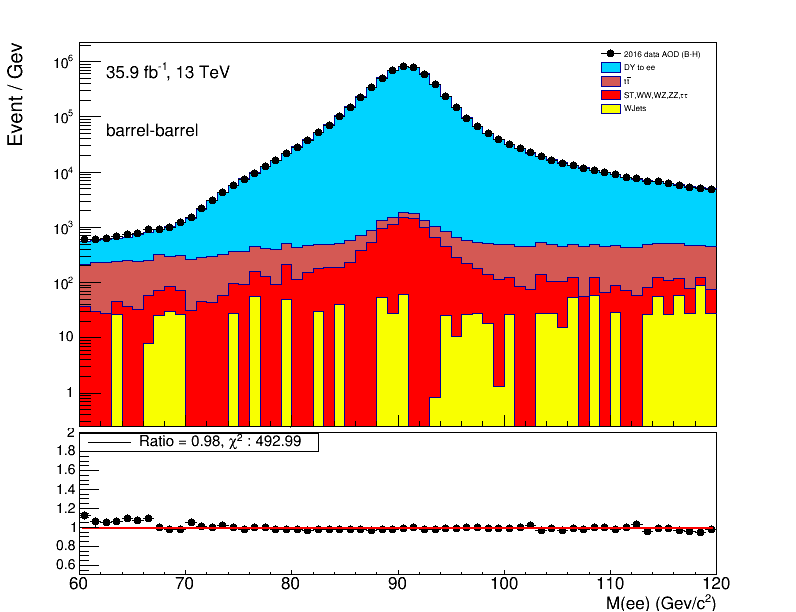
\includegraphics[angle=0,width=0.49\textwidth]{figures/Zprime/2016/zPeakDY/hratio_M_ee2__barrel-barrel.png}
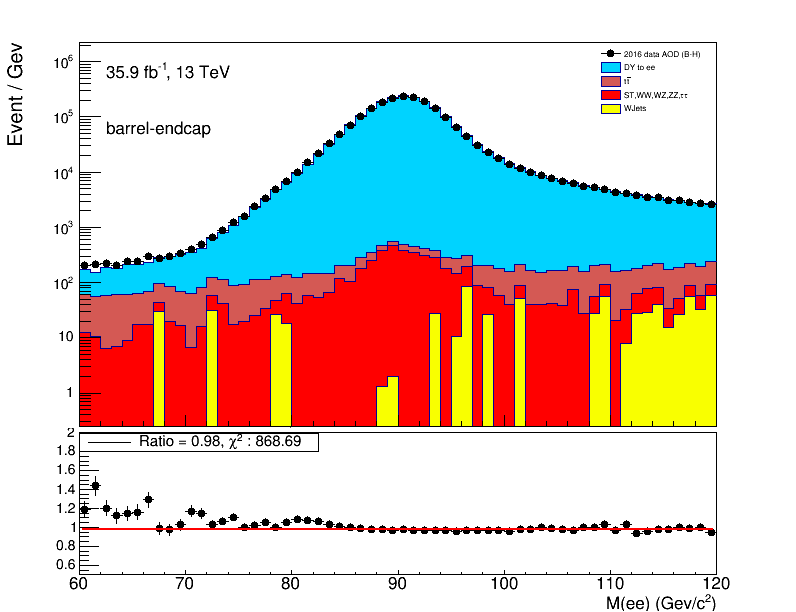
\includegraphics[angle=0,width=0.49\textwidth]{figures/Zprime/2016/zPeakDY/hratio_M_ee2__barrel-endcap.png}
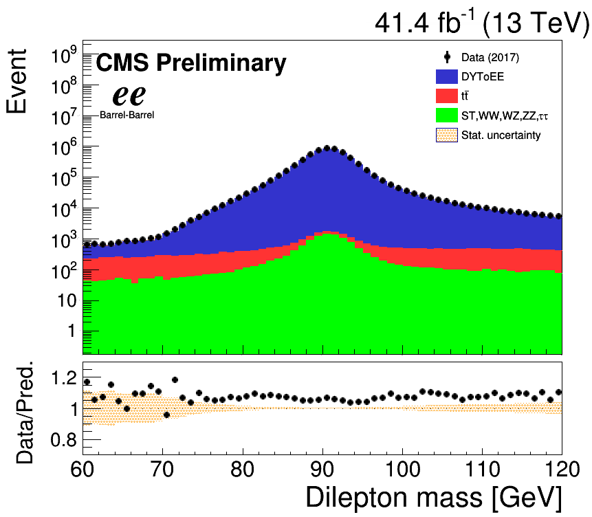
\includegraphics[angle=0,width=0.49\textwidth]{figures/Zprime/2017/zPeakDY/BB_hratio_M_ee.png}
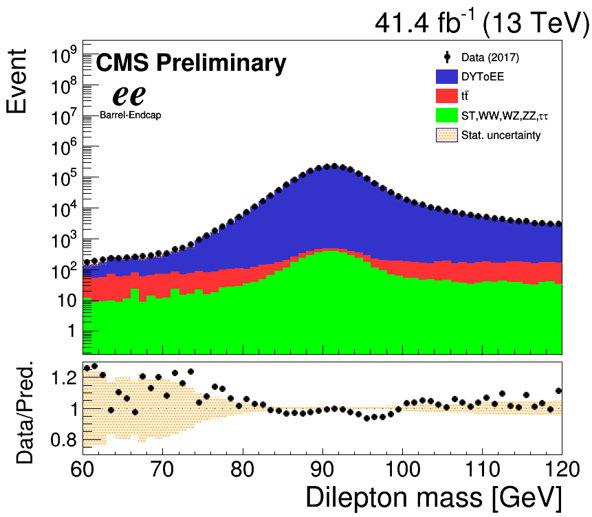
\includegraphics[angle=0,width=0.49\textwidth]{figures/Zprime/2017/zPeakDY/BE_hratio_M_ee.png}
\end{center}
\caption{Data - MC agreement in the Z peak region with the MC normalized to the luminosity of data for the barrel-barrel (left) and barrel-endcap (right) regions. The trigger turn on curve, gsf reconstruction and HEEP ID scale factor are applied for MC in 2016 (top) \cite{CMS-AN-2016-404} and 2017 (bottom) \cite{CMS-AN-2018-021}.}
\label{fig:Zpeak}
\end{figure}

A measured DY cross sections including the trigger efficiencies and data/MC efficiency scale factors are shown in Table~\ref{bkg:tab:zCrossSec}.
The SM DY cross section in mass range 60-120 GeV at NNLO is 1928$\pm72$ pb.
The measurement is in good agreement with the theory value. There is a $\sim$2\% difference for barrel-barrel region and a $\sim$0.3\% difference for barrel-endcap region in 2016. For 2017, it is $\sim$2\% for barrel-barrel region and $\sim$4\% for barrel-endcap region.
\begin{table}[!hbt]
\begin{center}
\resizebox{\linewidth}{!}{%
\begin{tabular}{|c|c|c|c|c|} \hline
Year                    & \multicolumn{2}{c|}{2016}                 & \multicolumn{2}{c|}{2017|} \\ \hline
Channel                 & barrel-barrel                     & barrel-endcap           & barrel-barrel                & barrel-endcap   \\\hline
N data events           & 5760345$\pm$2400                  & 2051759$\pm$1432        & 6189746$\pm$2488             & 2095959$\pm$1448\\
N expect bkg            & 32805                             & 11336                   & 32092                        & 10540           \\
MC acc$\times$eff       & 0.0880$\pm$0.001(stat.)           & 0.0315$\pm$0.001(stat.) & 0.0807$\pm$0.001(stat.)      & 0.0289$\pm$0.001(stat.)\\
Data/MC gsf RECO SF     & 0.979                             & 0.985                   &  -                           &  -                     \\
Data/MC HEEP ID Eff SF  & 0.943$\pm$0.001(stat.)            & 0.953$\pm$0.002(stat.)  & 0.935$\pm$0.002(stat.)       & 0.947$\pm$0.004(stat.) \\\hline
Luminosity (\invpb)     & 35867                             & 35867                   & 41368                        & 41368                  \\
DY cross-section (pb)   & 1967$\pm$3(stat)$\pm$51(lumi)     & 1922$\pm$3(stat)$\pm$50(lumi) & 1974$\pm$3(stat)       & 1854$\pm$3(stat)   \\\hline
Ratio to theory (1928 pb)&1.02                              &0.997                          &1.024                   &0.962                \\\hline
\end{tabular}}
\caption{Measurements of the DY cross section in the range of $\mathrm{60<M_{ee}<120}$ GeV. The scale factors for HEEP ID efficiency between data and MC are taken from Table~\ref{tab:HEEP_eff_nominal}.
It should be noticed that the scale factors in Table~\ref{tab:HEEP_eff_nominal} are for individual electrons, while here they are for electron pairs. For 2017, the gsf electron reconstruction efficiency scale factor between data and MC is already included in MC acc$\times$eff \cite{CMS-AN-2016-404,CMS-AN-2018-021}.}
\label{bkg:tab:zCrossSec}
\end{center}
\end{table}

\subsubsection{DY Background Correction and Uncertainty}
\label{sec:dyBkgCorr}
The main uncertainties on the Drell-Yan background originate from the parton density function (PDF) (which is the probability of finding a parton with a fraction $x$ of the proton momentum in the proton) and higher-order effects.
The cross-section has been evaluated using FEWZ 3.1.b2 with next-next-leading order (NNLO) accuracy in QCD and next-leading order (NLO) in electroweak (EWK).
Photon induced effects were taken into account by using a special PDF set, namely the LUXqed\_plus\_PDF4LHC15\_nnlo\_100.
Cross section ratios relative to the Z peak (60-120 GeV) were estimated together with their uncertainties by taking into account possible correlations
of the PDF uncertainties between the various mass bins. Full details of this calculation are in Ref. \cite{AN-16-053}.
The cross-sections in various mass bins were evaluated in the analysis acceptance ($\et>35$~GeV, $|\eta|<2.5$, excluding the $1.4442-1.566$ region).
The ratio of these cross-sections to that predicted by our POWHEG samples generated with NNPDF3.0 is shown in Figure~\ref{fig:fewzPowheg}.

%It is immediately noted that the POWHEG NNPDF3.0 prediction is increasingly higher than the FEWZ prediction at as the mass increases.
%This appears to be related to the choice of PDFs, figure~\ref{fig:fewzMCATNLOCTVsNNPDF3Powheg} shows the ratio pf the POWHEG cross-section
%predictions when using CT10 and C14 other the prediction using NNPDF3.0. It should be noted that ATLAS in their 2015 result used CT10.
%Finally the prediction of mc@NLO is compared to POWHEG is also shown in figure~\ref{fig:fewzMCATNLOCTVsNNPDF3Powheg}.

It is immediately noted that the POWHEG NNPDF3.0 prediction is increasingly higher than the FEWZ prediction as the mass increases.
In the analysis a FEWZ to POWHEG k-factor is applied.
This slightly improves data/MC agreement at high mass. The functional form for
this k-factor (accounting for the fact we normalize in the 60-120 GeV region) is shown
in Figure~\ref{fig:fewzPowheg}. This is now applied in the mass spectrum plots and the background estimations for the limits.

The PDF uncertainties for FEWZ 3.1.b2 with the LUXqed\_plus\_PDF4LHC15\_nnlo\_100 PDF set are shown in Table~\ref{bkg:tab:pdfUncert}.
The uncertainties quoted are on the DY cross section ratio of the invariant mass range considered to the Z peak region of 60 to 120 GeV. The uncertainties are fitted by polynomial which is shown in Figure \ref{fig:pdf_rel_uncert}.


\begin{figure}[bh]
\begin{center}
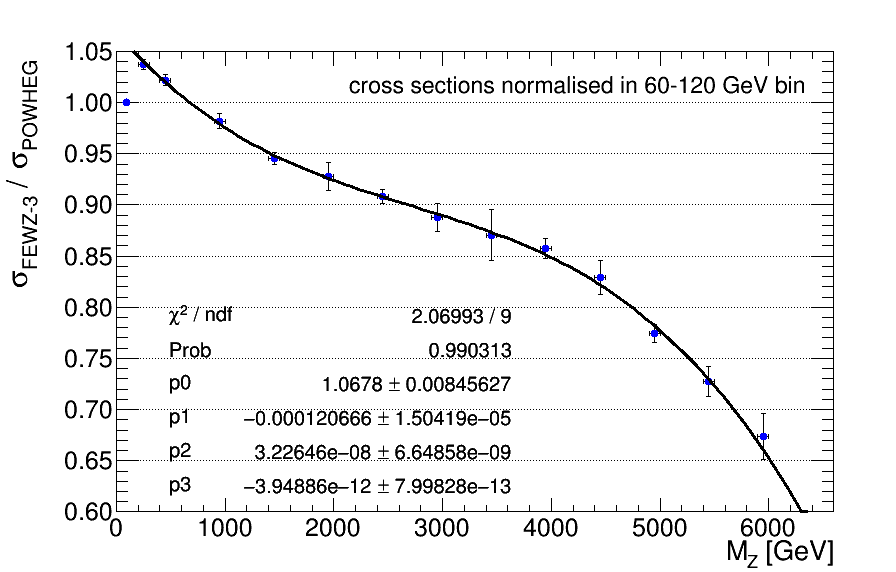
\includegraphics[angle=0,width=0.8\textwidth]{figures/Zprime/2016/zPeakDY/powhegFEWZKFactor.png}
\end{center}
\caption{
%The ratio of the \zee\ cross-section as predicted by FEWZ 3.1 at NNLO using the PDF4LHC15nnlo PDF set and that predicted by POWHEG at
%NLO using the NNPDF3.0 PDF set in various mass bins. The cross-sections are normalised to each other in the 60 to 120 GeV bin.
The ratio of the \zee cross-section as predicted by FEWZ 3.1.b2 using the LUXqed\_plus\_PDF4LHC15\_nnlo\_100 PDF set and that predicted by
POWHEG at NLO using the NNPDF3.0 PDF set in various mass bins. The cross-sections are normalized to each other in the 60 to 120 GeV bin \cite{CMS-AN-2016-404}.
}
\label{fig:fewzPowheg}
\end{figure}

%\begin{figure}[bh]
%\begin{center}
%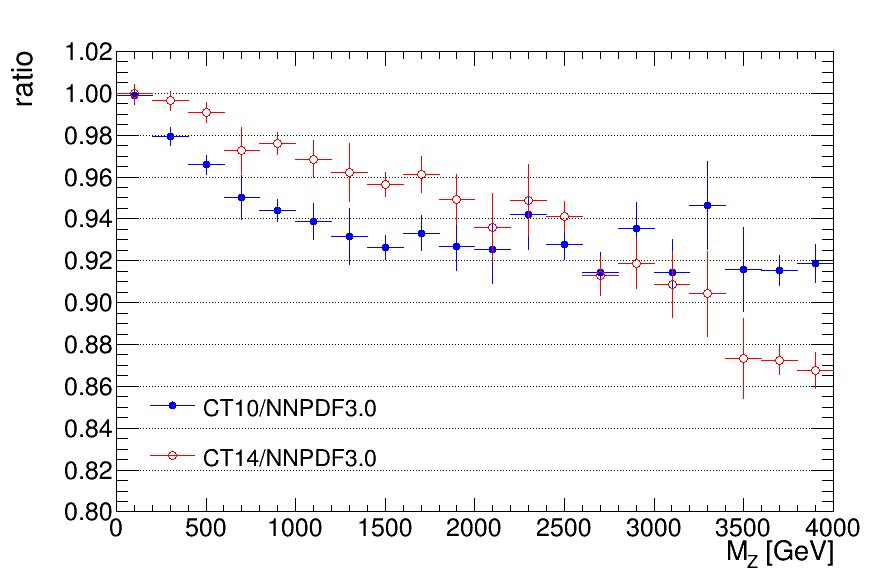
\includegraphics[angle=0,width=0.49\textwidth]{fig/fig_zPeakDY/ctOverNNPDF.png}
%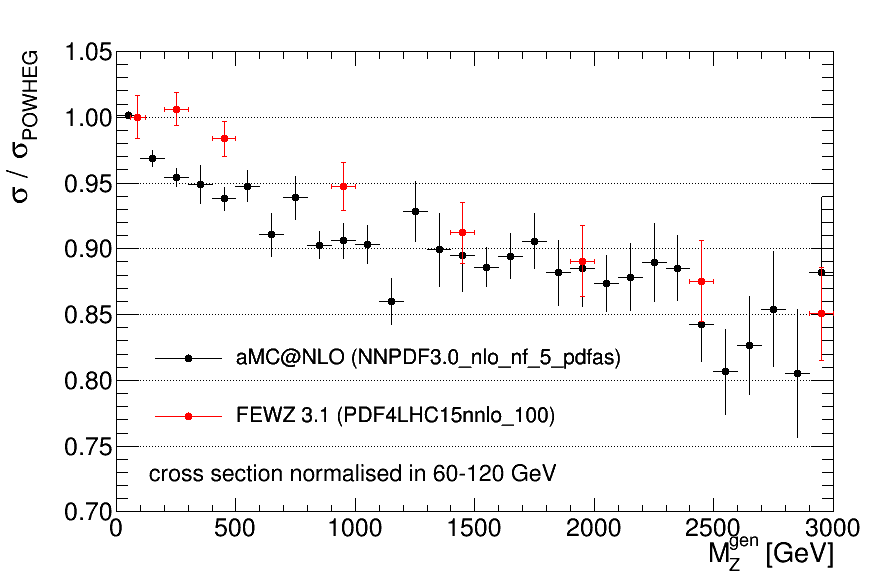
\includegraphics[angle=0,width=0.49\textwidth]{fig/fig_zPeakDY/mcatnloFewzVsPowheg}
%\end{center}
%\caption{
%The ratio of the \zee\ cross-section as predicted by FEWZ 3.1 at NNLO using the PDF4LHC15nnlo PDF set
%and as predicted by mc@NLO at NLO using the NNPDF3.0 PDF set to that predicted by POWHEG at NLO using the
%NNPDF3.0 PDF set in various mass bins. All cross-sections normalised to each other in the 60 to 120 GeV bin.
%}
%\label{fig:fewzMCATNLOCTVsNNPDF3Powheg}
%\end{figure}


\begin{table}[t]
\begin{center}
\smallskip\noindent
%\resizebox{\linewidth}{!}{%
\begin{tabular}{|c|c|} \hline
Mass range (GeV) & Relative uncertainty \\\hline
 200-300 & 1.21\% \\
 400-500 & 1.54\% \\
900-1000 & 2.16\% \\
1400-1500 & 2.73\% \\
1900-2000 & 3.24\% \\
2400-2500 & 3.72\% \\
2900-3000 & 4.27\% \\
3400-3500 & 5.00\% \\
3900-4000 & 5.94\% \\
4400-4500 & 7.47\% \\
4900-5000 & 10.2\% \\
5400-5500 & 14.3\% \\
5900-6000 & 19.9\% \\\hline
\end{tabular}%}
\caption{The PDF uncertainties on the DY cross section relative to the Z boson peak region (60-120 GeV) as a function of mass \cite{CMS-AN-2016-404}.
%These numbers are taken from Table 3 of AN-16-053 v3~\cite{AN-16-053}
}
\label{bkg:tab:pdfUncert}
\end{center}
\end{table}

\begin{figure}[bh]
\begin{center}
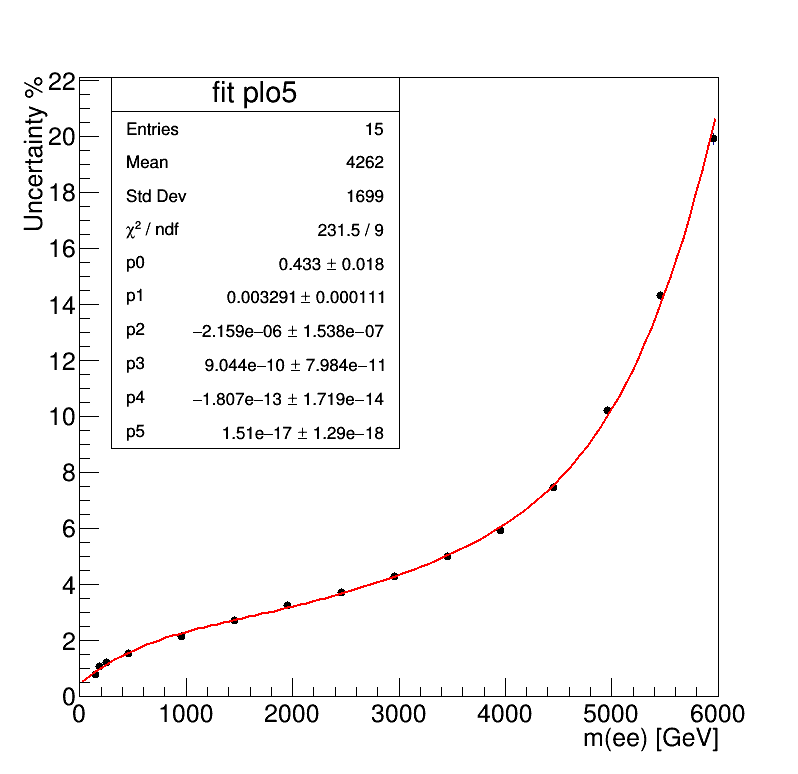
\includegraphics[angle=0,width=0.8\textwidth]{figures/Zprime/2016/pdf_uncert_relative.png}
\end{center}
\caption{
The PDF uncertainties on the DY cross section relative to the Z peak region as a function of dielectron invariant mass.
}
\label{fig:pdf_rel_uncert}
\end{figure}



\clearpage
